\documentclass[border=3mm]{standalone}

\usepackage{pgfplots}
\pgfplotsset{height=5cm,width=10cm,compat=1.15}

\begin{document}

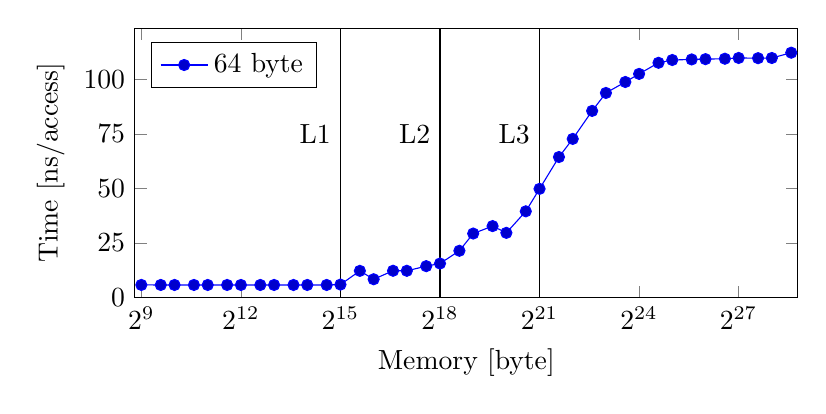
\begin{tikzpicture}
\begin{axis}[
	xmode=log,
	log basis x={2},
	ylabel={Time [ns/access]},
	xlabel={Memory [byte]},
	%scaled ticks=false,
	y tick label style={/pgf/number format/fixed},
	x tick label style={/pgf/number format/fixed},
	ytick distance={25},
	ymin = 0,
	%xmin = 64,
	enlarge x limits=0.01,
	legend style={at={(0.15, 0.95)}, anchor=north,legend columns=1},
	%ybar,
	% xtick=data,
	% bar width=7pt,
]
\addplot table {
512     5.719585352     134217728
768     5.704017423     134217728
1024    5.703802437     134217728
1536    5.704475924     134217728
2048    5.698261574     134217728
3072    5.697355591     134217728
4096    5.700166091     134217728
6144    5.697381921     134217728
8192    5.704047561     134217728
12288   5.697260186     134217728
16384   5.703742325     134217728
24576   5.699306123     134217728
32768   5.875355959     134217728
49152   12.169322833    134217728
65536   8.325341888     134217728
98304   12.210437916    134217728
131072  12.200340584    134217728
196608  14.327157803    134217728
262144  15.535811856    134217728
393216  21.384247378    134217728
524288  29.286882102    134217728
786432  32.700426340    134217728
1048576 29.599094056    134217728
1572864 39.475372821    134217728
2097152 49.781680524    134217728
3145728 64.377416991    134217728
4194304 72.690074578    134217728
6291456 85.527437814    134217728
8388608 93.758271061    134217728
12582912        98.789244942    134217728
16777216        102.499310598   134217728
25165824        107.593063243   134217728
33554432        108.872263901   134217728
50331648        109.129389726   134217728
67108864        109.269013643   134217728
100663296       109.456830002   134217728
134217728       109.807311513   134217728
201326592       109.711245567   134217728
268435456       109.790928833   134217728
402653184       112.223176248   134217728
};
%\addplot coordinates {(O0,0.034254) (O1,0.062424) (O2,4.4731) (O3,4.4157)};
\draw (32768,0) -- node[left]{L1} (32768, 150);
\draw (262144,0) -- node[left]{L2} (262144, 150);
\draw (2097152,0) -- node[left]{L3} (2097152, 150);


%\node[above] at (axis cs:O0,0.03177) {$\sim$0.03};
%\node[above] at (axis cs:O1,0.060008) {$\sim$0.06};

\legend{64 byte}
\end{axis}
\end{tikzpicture}

\end{document}
